\documentclass[10pt]{article}
\usepackage{fullpage}
\usepackage{tikz}

\usetikzlibrary{shapes.geometric, arrows}

\tikzstyle{file} = [rectangle, rounded corners, minimum width=3cm, minimum height=1cm, text centered, text width=3cm, draw=black]
\tikzstyle{fileL} = [rectangle, rounded corners, minimum width=3cm, minimum height=1cm, text centered, text width=4cm, draw=black]
\tikzstyle{folder} = [rectangle, minimum width=3cm, minimum height=1cm, text centered, text width=3cm, draw=black]
\tikzstyle{arrow} = [thick, ->, >=stealth]

\begin{document}

\title{\vspace{-2cm}ARM Checkpoint - Group 16}
\author{\small Ayoob Ahmed, Aayush Dalal, Al-Maz Ahmad, Devam Savjani}


\maketitle

This report describes how we are working in a group and how we have gone about the ARM11 emulator. Working in group have proven difficult considering we cannot meet in person however we have been able to mitigate this problem by using various online platforms including Whatsapp and Discord.
\section{Group Organisation}
\subsection{Delegation of Workload}
In order to split the workload evenly and more efficiently, we initially discussed how we can go about the task. We debated on particular approaches we could take, eventually agreeing on one. From that initial meeting we each took away something to do, from then on we split work in terms of functions that we would need to create. To begin with we considered the data types we would need to implement, considering that we may need more as the project continues. 
\\By splitting each individual function, for example, the execution of the instruction, as the instructions could be any from 4 types we split the four types between us. We were aware of the fact that some types would require more work than others, and thus we decided that when those working on the quicker functions, they would then assist those working on the longer ones for example data processing instructions. We constantly use our Whatsapp group-chat and frequently speak on Discord to review our tasks. Having the Discord server helped us keep track of the tasks yet to be completed , tasks completed and the status of the task which was very useful to delegate the work in an even manner.
\subsection{The Group Dynamic}
In terms of our group dynamic and how we are working in a team, we think our team is working well constantly communicating on our whereabouts of each of our sub-tasks. To begin with although we discussed what we had to do, we still experienced a rocky start, some of us were confused about how to start and drifted apart. However, we immediately noticed that going our separate ways would not work to produce a complete and efficient code and thus from then on we began to discuss on our successes and problems we had faced daily so that we would be able to communicate what is left to be done. In this way, despite the start, we have become stronger and more efficient in working as a team. 
 This approach by talking to each other every day to update each other helps us as if someone is very unsure about their task, we can swap tasks to have a someone who understands the problem to find the best possible solution and approach. As the part 1 of the project came to a close, when all of the functions were finished, we assigned two people to string the functions together and the other two to begin working on the second part. We thought this would be reasonable so that not much work would need to be done to do this and ensure all of the test cases are working. After splitting up into two groups, we completed the testing and stringing everything together we went back to complete the optional task and attempt to make the program more efficient and get rid of any unnecessary code.
\\In the beginning, we also faced another problem in which certain periods some members would not be able to work even though when we were able to work we were communicating well. To overcome this issue, we created a log type system on our discord server such that if someone would be unable to work on the project for a day, the other team members are aware of what has been done and what is yet to be completed.

\section{Implementation Strategies}
\subsection{Structure of our Emulator}
To represent our ARM system we created a struct which contains a pointer to memory, an array of type unsigned 32-bit integer of size 17.. It also contains an array that stores two booleans; one which states whether an instruction has been fetched and the other if it has been decoded. We created an {\tt{emulator\_utils}} directory which that contains the {\tt{defines.h}} file and the other helper functions to help the execution of the instruction. The structure of our emulator is as follows:

\begin{itemize}
	\item {\tt{emulate.c}} - contains the function {\tt{main}} which reads the input binary file then passes the data onto the pipeline in order to execute the instruction. The file also uses the {\tt{emulator\_utils\textbackslash defines.h}} header which contains all of the necessary constants, libraries, data types, enums, and the decelerations of the functions that need to be used.
	\item {\tt{decodeInstr.c}} - as we initially decided to have the struct to contain the big-endian instruction due to the fact that the instructions in the file are written in little-endian, therefore in order to carry out this process we implemented this file that carries out this process for us.
	\item {\tt{executeInstr.c}}, {\tt{executeHelper.c}} and {\tt{shiftInstruction.c}} - these three files execute the instruction where the {\tt{executeInstr.c}} file finds out the type of the instruction and then executes it with its corresponding execute function, found in {\tt{executeHelper.c}}. The {\tt{shiftInstruction.c}} file contains all of the types of the shifts and has their execution functions for all of them which helps the {\tt{executeHelper.c}} with the execution of the instruction.
	\item {\tt{pipeline.c}} and {\tt{output.c}} - to simulate the three-stage pipeline, we implemented a function to carry out the process, which is found in the {\tt{pipeline.c}} file. The {\tt{output.c}} outputs the result statuses of the registers such that it prints the value of each register and the contents of any non-zero memory locations.
	
\end{itemize}


The diagram below shows the structure the emulate file, we created a directory {\tt{emulator\_utils}} to store all of the helper functions. Within the directory, the {\tt{defines.h}} header declares all of the constants and functions.
\begin{center}

\scalebox{0.8}{
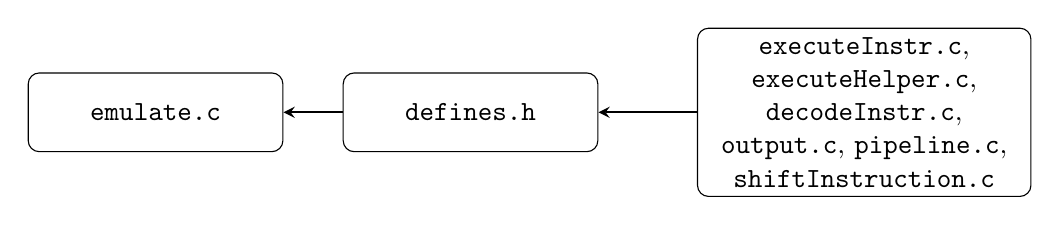
\begin{tikzpicture}[node distance=1cm]
\node (emulate) [file] {{\tt{emulate.c}}};
%\node (emulator_utils) [folder, right of=emulate, xshift=3cm] {{\tt{emulator\_utils}}};
\node (defines) [file, right of=emulate, xshift=3cm] {{\tt{defines.h}}};
\node (other) [fileL, right of=defines, xshift=4cm] {{\tt{executeInstr.c}}, {\tt{executeHelper.c}}, {\tt{decodeInstr.c}}, {\tt{output.c}}, {\tt{pipeline.c}}, {\tt{shiftInstruction.c}}};
\draw [arrow] (other) -- (defines);
\draw [arrow] (defines) -- (emulate);
%\draw [arrow] (emulator_utils) -- (emulate);
\end{tikzpicture}}
\end{center}


\subsection{The Future of our Project}
From the Emulator part, we potentially may use the endian converter to convert the instructions from big-endian to little-endian and the constants we had defined in the {\tt{defines.h}} file. Hence reducing the number of magic numbers. For debugging purposes, we also use the {\tt{output.c}} file to help us print the status of the registers as the instructions are being executed. We will have the {\tt{main}} in {\tt{assemble.c}} and we hope to structure the programs in a similar way as we structured our {\tt{emulate.c}}.
\\After discussing the second part of the project, we discussed how we could implement the symbol table. Speaking about different approaches including heaps, binary trees and some others are helping us decide in the best approach we can implement, debating each of the pros and cons of each approach helped us choose an approach that would be efficient. Writing the benefits and drawbacks of each of the approaches will help us later on when implementing the ADT as we would have a clear view of the task to avoid any confusion in the task.
\\Another aspect of the task, we discussed was the tokenizer we mitigated this by discussing different approaches in the same way as we did with the ADT. We conducted some more research as a group together to fill up gaps in our knowledge as a group so that we could use our research to help us work more efficiently.

\end{document}
